\documentclass{article}
\usepackage{xcolor}
\usepackage{ragged2e}
\usepackage{graphicx}
\usepackage{subcaption}
\graphicspath{ {./sdcard/Download/fwc/} }

\begin{document}

\begin{center}
	\color{blue} CHAPTER 7: TRIANGLES
\end{center}
\begin{center}
	\color{blue} EXERCISE 7.3
\end{center}

\begin{enumerate}
\item $ABC$ is an isosceles triangle with $AB=AC$ and $BD$ and $CE$ are its two medians. Show that $BD=CE$.
\item In Fig.7.4, $D$ and $E$ are the points on side $BC$ of a $\triangle ABC$ such that $BD=CE$ and $AD=AE$. Show that $\triangle ABD \cong \triangle ACE$.
\begin{figure}[h]
	\centering
	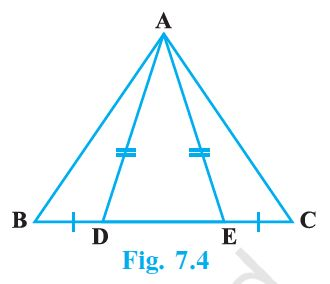
\includegraphics[scale=0.5]{Figure1}
\end{figure}
\item $CDE$ is an equilateral triangle formed on a side $CD$ of a square $ABCD$ (Fig.7.5). Show that $\triangle ADE \cong \triangle BCE$.
\begin{figure}[h]
	\begin{subfigure}{0.5\textwidth}
		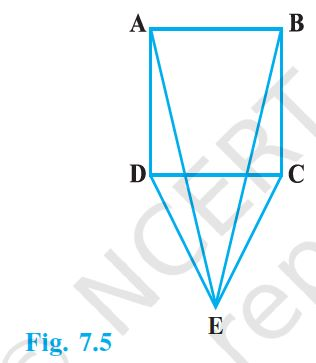
\includegraphics[width=0.9\linewidth,scale=0.5]{Figure2}
	\end{subfigure}
	\begin{subfigure}{0.5\textwidth}
		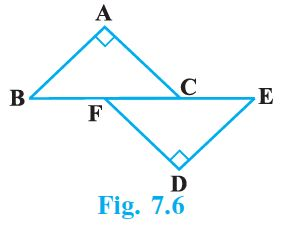
\includegraphics[width=0.9\linewidth,scale=0.5]{Figure3}
	\end{subfigure}
\end{figure}
\item In Fig.7.6, $BA \perp AC$, $DE \perp DF$ such that $BA=DE$ and $BF=EC$. Show that $\triangle ABC \cong \triangle DEF$.
\item $Q$ is a point on the side $SR$ of $\triangle PSR$ such that $PQ=PR$. Prove that $PS>PQ$.
\item $S$ is any point on side $QR$ of a $\triangle PQR$. Show that $PQ+QR+RP>2PS$.
\item $D$ is any point on side $AC$ of a $\triangle ABC$ with $AB=AC$. Show that $CD<BD$.
\item In Fig.7.7, $l \| m$ an $M$ is the mid-point of a line segment $AB$. Show that $M$ is also the mid-point of any line segment $CD$, having its end points on $l$ and $m$, respectively.
\item Bisectors of the $\angle B$ and $\angle C$ of an isosceles triangle with $AB=AC$ intersect each other at O. BO is produced to a point $M$. Prove that $\angle MOC= \angle ABC$.
\begin{figure}[h]
	\begin{subfigure}{0.5\textwidth}
		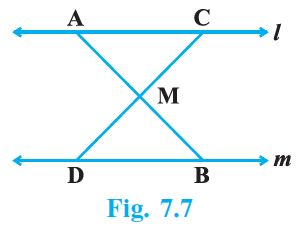
\includegraphics[width=0.9\linewidth,scale=0.5]{Figure4}
	\end{subfigure}
	\begin{subfigure}{0.5\textwidth}
		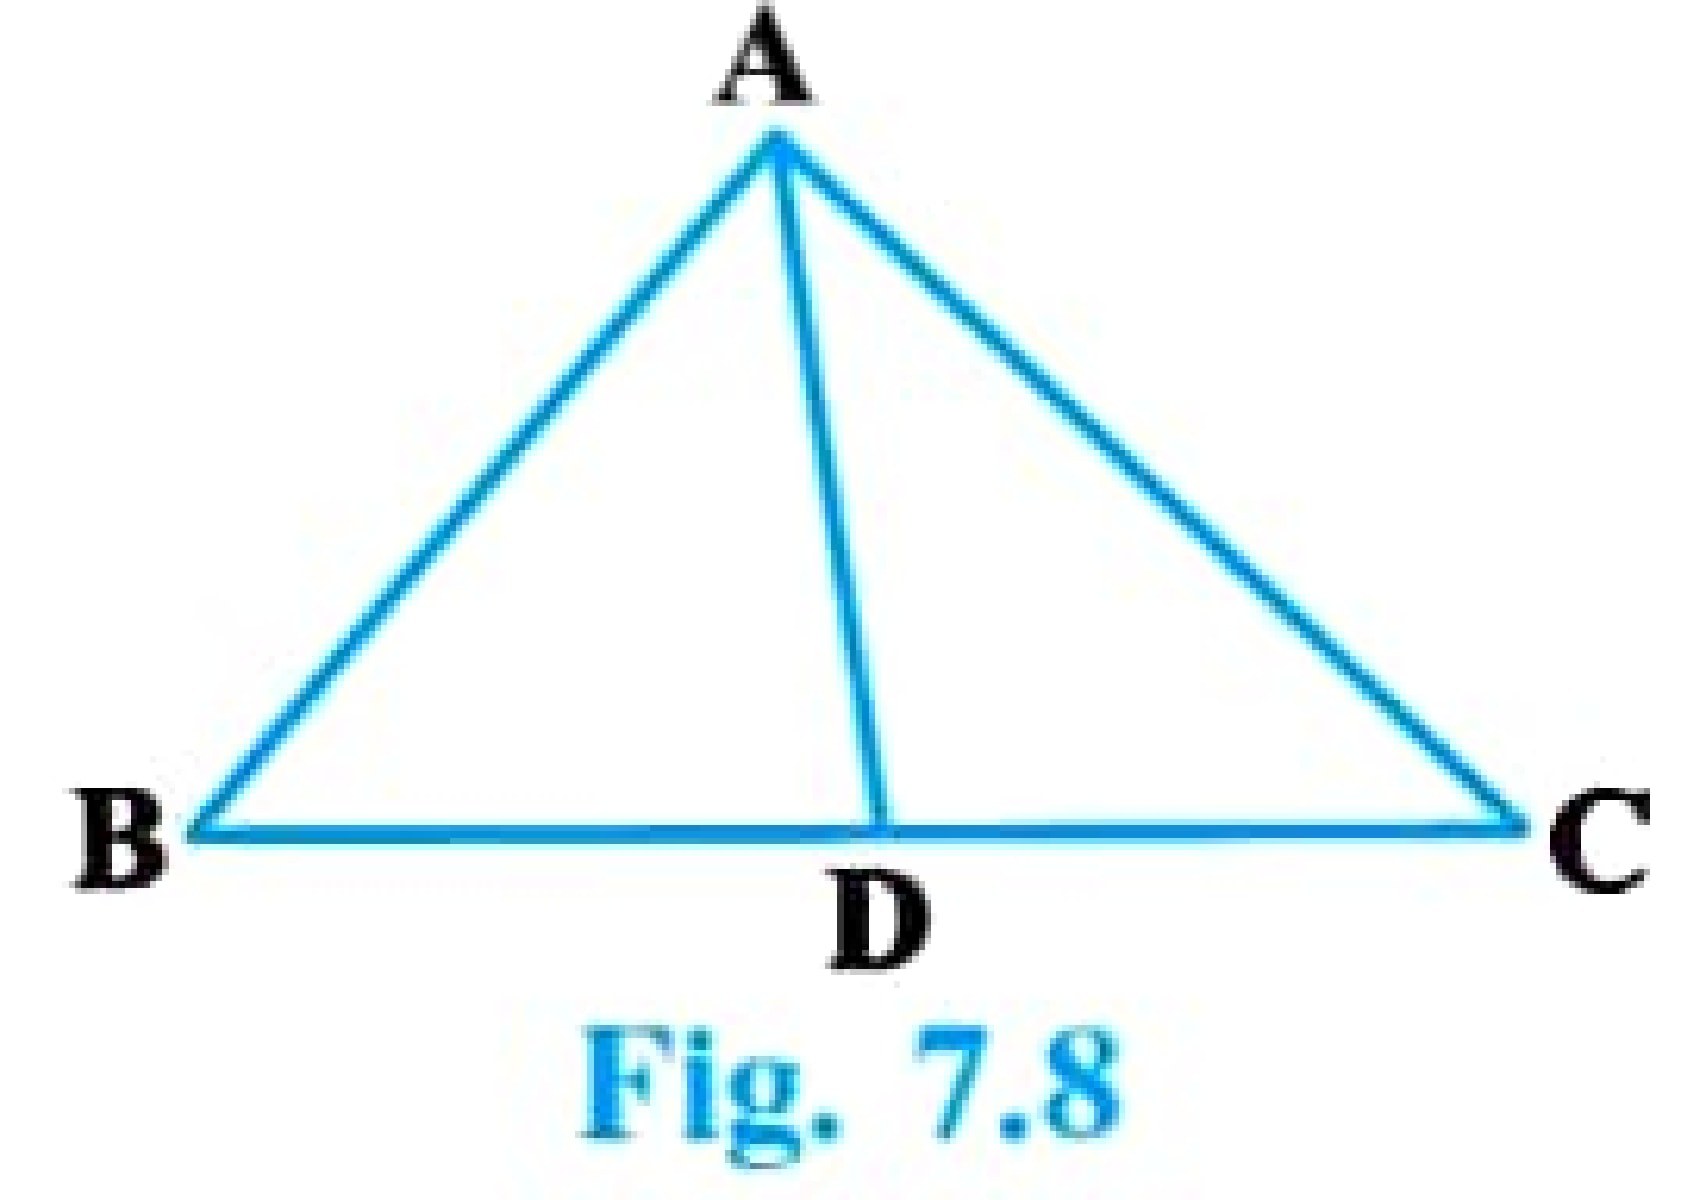
\includegraphics[width=0.9\linewidth,scale=0.08]{Figure5}
	\end{subfigure}
\end{figure}
\item Bisectors of the $\angle B$ and $\angle C$ of an isosceles triangle $ABC$ with $AB=AC$ intersect each other at $O$. Show that the external angle adjacent to $\angle ABC$ is equal to $\angle BOC$.
\item In Fig.7.8, $AD$ is the bisector of $\angle BAC$. Prove that $AB>BD$.
\end{enumerate}
\end{document}
